\documentclass{beamer}
\usepackage{amsfonts,amsmath,oldgerm}
\usepackage{ragged2e}
\usepackage{amsfonts}
\usepackage{amsmath}
\usetheme{sintef}

\newcommand{\testcolor}[1]{\colorbox{#1}{\textcolor{#1}{test}}~\texttt{#1}}

\usefonttheme[onlymath]{serif}

\titlebackground*{assets/background}

\newcommand{\hrefcol}[2]{\textcolor{cyan}{\href{#1}{#2}}}

\title{Aula 02 - Single Page Applications}
\subtitle{2023.1 - PDWA5 - Programação Dinâmica para Web}
\course{Tecnologia em Análise e Desenvolvimento de Sistemas}
\author{\href{mailto:luiz.quirino@ifsp.edu.br}{Luiz \textbf{Quirino}}}
\IDnumber{luiz.quirino@ifsp.edu.br}



\begin{document}
\maketitle

%\begin{frame}
%
%      Este material é produzido utilizando \LaTeX\, baseado na SINTEF Presentation, disponibilizado sob licenciamento \hrefcol{https://creativecommons.org/licenses/by-nc/4.0/legalcode}{Creative Commons CC BY 4.0}
%
%\vspace{\baselineskip}

%In the following you find a brief introduction on how to use \LaTeX\ and the beamer package to prepare slides, based on the one written by \hrefcol{mailto:federico.zenith@sintef.no}{Federico Zenith} for \hrefcol{https://www.overleaf.com/latex/templates/sintef-presentation/jhbhdffczpnx}{SINTEF Presentation}

% This template is released under \hrefcol{https://creativecommons.org/licenses/by-nc/4.0/legalcode}{Creative Commons CC BY 4.0} license
%\end{frame}
\footlinecolor{maincolor}
\section{introdução}
\begin{frame}
      \frametitle{Aplicações de Uma Única Página (SPA)}
      \begin{itemize}
            \item A lógica da aplicação é executada no navegador.
            \item Fornece uma experiência de usuário mais semelhante a um desktop.
            \item As solicitações HTTP são tratadas de forma assíncrona (e de maneira discreta).
            \item A navegação tradicional é geralmente desencorajada.
      \end{itemize}
\end{frame}

\begin{frame}
      \frametitle{Funcionamento Interno e Arquitetura}
      \begin{itemize}
            \item Tratado internamente alterando o DOM dinamicamente.
            \item Arquitetura de servidor enxuta.
            \item Armazenamento de dados, verificações de segurança, etc.
      \end{itemize}
\end{frame}

\begin{frame}
      \frametitle{Desvantagens}
      \begin{itemize}
            \item Inicialização da aplicação - tempo de carregamento e inicialização.
            \item Ambiente de execução menos estável (vários tipos de navegadores).
      \end{itemize}
\end{frame}

\begin{frame}
      \frametitle{Thick client e Thin Server}
      \begin{itemize}
            \item HTTP não é mais utilizado (apenas) no sentido tradicional.
            \item Conceito tipo RPC(Chamada de Procedimento Remoto) é utilizado sobre HTTP ou WebSockets.
            \item O servidor executa apenas as operações que não podem ou não devem ser transferidas para o cliente.
      \end{itemize}
\end{frame}

\begin{frame}
      \frametitle{Gestão de Dados e Autenticação}
      \begin{itemize}
            \item Gerenciamento de dados (recuperação, modificações, …).
            \item Dados são transferidos em JSON ou em formato nativo (imagens).
            \item Autenticação e autorização.
      \end{itemize}
\end{frame}

\begin{frame}
      \frametitle{Base de Computação Confiável e Tarefas de Suporte}
      \begin{itemize}
            \item A base de computação confiável não pode ser estendida ao cliente.
            \item Tarefas de suporte:
                  \begin{itemize}
                        \item Fornecendo módulos, estilos, …
                        \item Pré-renderização de fragmentos de HTML (otimização de performance).
                  \end{itemize}
      \end{itemize}
\end{frame}
\begin{frame}
      \frametitle{Transferência de Estado Representacional (REST)}
      \begin{itemize}
            \item Recursos são identificados por URIs.
                  \begin{itemize}
                        \item /galeria – todas as galerias.
                        \item /galeria/2017 – uma galeria.
                        \item /galeria/2017/gatinho1 – uma fotografia.
                  \end{itemize}
      \end{itemize}
\end{frame}

\begin{frame}
      \frametitle{Operações via Requisições HTTP}
      \begin{itemize}
            \item O método de requisição determina a operação.
      \end{itemize}
\end{frame}

\begin{frame}
      \frametitle{Conceito CRUD}
      \begin{itemize}
            \item Criar, Ler, Atualizar, Deletar.
            \item Corresponde aos métodos HTTP POST, GET, PUT, DELETE.
            \item Operações mais básicas de armazenamento de dados.
      \end{itemize}
\end{frame}


\begin{frame}
      \frametitle{Problemas de Design em SPAs}

      \begin{itemize}
            \item \textbf{Inadequação do HTML}
                  \begin{itemize}
                        \item O HTML não foi feito para ser usado em páginas dinâmicas.
                        \item HTML é enviado pelo servidor e também modificado via DOM.
                  \end{itemize}

            \item \textbf{Dificuldade em rastrear o estado da IU}
                  \begin{itemize}
                        \item Normalmente, o DOM não pode manter todo o estado da aplicação (por exemplo, transferências AJAX pendentes).
                        \item O problema raiz das aplicações SPA.
                  \end{itemize}

            \item \textbf{Mistura de Mutação e Assincronicidade}
                  \begin{itemize}
                        \item Estado (e IU) precisa mudar.
                        \item A mudança é iniciada por ações assíncronas.
                        \item Eventos do usuário, eventos de rede, temporizadores, ...
                  \end{itemize}
      \end{itemize}

\end{frame}

\begin{frame}
      \frametitle{Problemas no Desenvolvimento Frontend}

      \begin{itemize}
            \item \textbf{Compatibilidade do Navegador}
                  \begin{itemize}
                        \item Muitos fornecedores e versões de navegadores.
                        \item Javascript (Ecmascript) evolui rapidamente.
                        \item Existem extensões/modificações de scripts.
                        \item TypeScript, JSX, ...
                  \end{itemize}

            \item \textbf{Polyfill}
                  \begin{itemize}
                        \item Preenche com novos recursos (novos objetos, funções, APIs, ...) em versões antigas de ES.
                  \end{itemize}

            \item \textbf{Transpiladores}
                  \begin{itemize}
                        \item Compiladores de ES mais recente ou outra linguagem para ES5.
                        \item Podem ser executados dinamicamente, ou o projeto precisa ser compilado antes da implantação.
                  \end{itemize}
      \end{itemize}

\end{frame}

\begin{frame}
      \frametitle{Eventos e Ações do Usuário}

      \begin{itemize}
            \item \textbf{Eventos do Usuário Estão Ligados à Estrutura DOM}

            \item \textbf{Ações do Usuário São Abstratas} (não vinculadas ao DOM)

            \item \textbf{Um Evento Pode Acionar uma Ação que não Está Relacionada ao DOM}

            \item \textbf{Mecanismo para Processamento Global de Ações}
      \end{itemize}

\end{frame}

\begin{frame}
      \frametitle{Componentes}

      \begin{itemize}
            \item \textbf{Uma Forma Inteligente de Dividir o Código}

            \item \textbf{Os Componentes Precisam se Comunicar/Cooperar}

            \item \textbf{Componentes Podem Competir por Recursos}
                  \begin{itemize}
                        \item Armazenamento local, trabalhadores (workers), ...
                  \end{itemize}
      \end{itemize}

\end{frame}

\begin{frame}
      \frametitle{Separe Estado e Apresentação}

      \begin{itemize}
            \item \textbf{O estado é armazenado em um objeto separado (estrutura)}

            \item \textbf{O DOM é atualizado quando o estado muda}
                  \begin{itemize}
                        \item Associações de dados (DOM – estado)
                        \item (parcial) Re-renderização do DOM
                  \end{itemize}

            \item \textbf{Eventos DOM podem acionar mudanças de estado}

            \item \textbf{Associação de dados bidirecional}

            \item \textbf{Eventos emitem ações}

            \item \textbf{Questão de mutabilidade do estado}
                  \begin{itemize}
                        \item Estado mutável monitorado por observadores
                        \item Estado imutável (novo estado deve ser construído)
                  \end{itemize}
      \end{itemize}

\end{frame}




\begin{frame}
      \frametitle{SPA vs. Aplicações Desktop}

      \begin{itemize}
            \item \textbf{Conceitos de Interface de Usuário Similares}

            \item \textbf{Programação Orientada a Eventos}

            \item \textbf{Ambiente e Segurança}
                  \begin{itemize}
                        \item É muito mais simples hackear o código de uma aplicação web do que uma aplicação desktop comum (compilada).
                  \end{itemize}

            \item \textbf{Comunicação com o Servidor}
                  \begin{itemize}
                        \item Um atributo definidor das aplicações web.
                        \item Outra(s) fonte(s) de erros em tempo de execução.
                        \item Erros do lado do servidor, erros de comunicação, timeouts, ...
                        \item Solicitações assíncronas podem interferir com eventos de interface de usuário.
                  \end{itemize}
      \end{itemize}

\end{frame}

\section{Arquitetura e paradigmas}

\begin{frame}{MVC - Cliente - Servidor}

      \begin{center}
            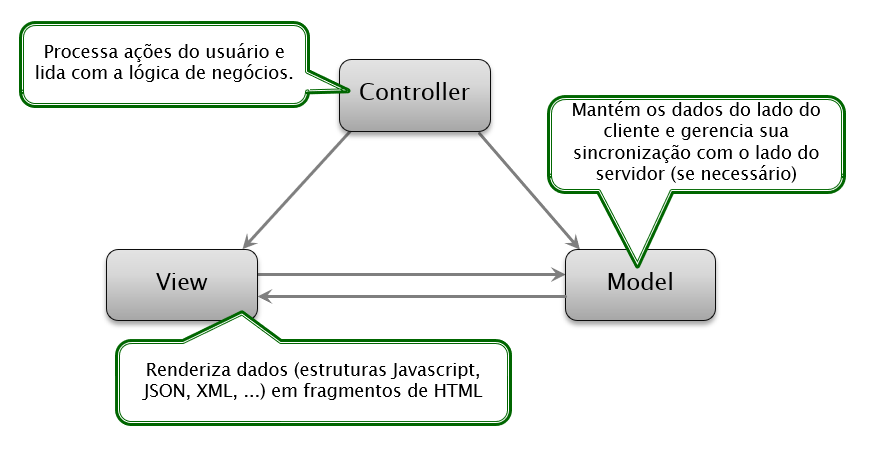
\includegraphics[width=0.8\linewidth]{assets/aula-tads-pdwa5/mv-client-side.png}
      \end{center}
\end{frame}

\begin{frame}
      \frametitle{Modelo-Visão-ViewModel (MVVM)}

      \begin{itemize}
            \item \textbf{Simplifica a apresentação de dados, especialmente em SPA (Single Page Applications)}
      \end{itemize}
      \begin{center}
            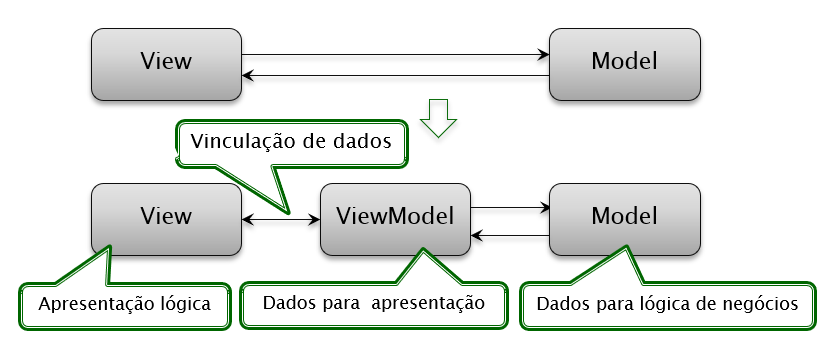
\includegraphics[width=0.8\linewidth]{assets/aula-tads-pdwa5/mvvm.png}
      \end{center}
\end{frame}

\section{Conceitos e Frameworks}
\begin{frame}
      \frametitle{Biblioteca AngularJS}

      \begin{itemize}
            \item \textbf{Framework SPA de código aberto, impulsionado pelo Google}
            \item \textbf{Adota os padrões MVC e MVVM}
            \item \textbf{Lógica nos controladores é codificada de forma imperativa}
            \item \textbf{Ligações de dados são declarativas (embutidas no HTML)}
            \item \textbf{Objeto \$scope - um contexto para a maioria das operações}

      \end{itemize}

\end{frame}
\begin{frame}
      \frametitle{Biblioteca AngularJS}

      \begin{itemize}
            \item \textbf{Variáveis do scope podem ser vinculadas a fragmentos de página}
            \item \textbf{Ligação de dados bidirecional}
            \item \textbf{Atualizações são realizadas de forma iterativa (ciclo digest)}
            \item \textbf{Angular 2 lançado recentemente}
            \item \textbf{Reescrita completa, muitas mudanças}
            \item \textbf{Microsoft TypeScript - versão tipada do Javascript}
      \end{itemize}

\end{frame}

\begin{frame}
      \frametitle{Biblioteca AngularJS}

      \begin{itemize}
            \item \textbf{MVVM e Ligação de Dados}
            \item \textbf{Declarativo, embutido no HTML}
            \item \textbf{Tipicamente como novos atributos e classes CSS}
                  \\ \texttt{<input type="text" ng-model="caption">}
            \item \textbf{Usando uma sintaxe especial diretamente no conteúdo do texto}
                  \\ \texttt{<p>Nome do Usuário: \{\{ firstName \}\} \{\{ lastName \}\}</p>}
      \end{itemize}

\end{frame}

\begin{frame}
      \frametitle{Biblioteca AngularJS}

      \begin{itemize}
            \item \textbf{O Viewmodel é o contexto \$scope}
            \item \textbf{As ligações são bidirecionais}
            \item \textbf{Automaticamente propagadas em ambos os sentidos}
            \item \textbf{\$scope.caption ←→ input.value (como acima)}
            \item \textbf{\$scope.firstName → renderizado para o espaço reservado do texto}
            \item \textbf{O controlador trabalha apenas com o objeto \$scope}
      \end{itemize}

\end{frame}

\begin{frame}
      \frametitle{Biblioteca AngularJS}

      \begin{itemize}
            \item \textbf{Diretivas}
            \item Muitas diretivas embutidas para controle visual
            \item ng-bind, ng-model
            \item ng-if, ng-switch, ng-repeat, ng-show, ng-hide
            \item Definindo diretivas personalizadas
      \end{itemize}

\end{frame}

\begin{frame}
      \frametitle{Biblioteca AngularJS}

      \begin{itemize}
            \item \textbf{Controladores}
            \item Realiza a inicialização do \$scope
            \item Declare funções (ações), que podem ser acionadas por manipuladores de eventos (por exemplo, ng-click)
      \end{itemize}

\end{frame}
\begin{frame}
      \frametitle{MVC e Escalabilidade de Recursos}

      \begin{itemize}
            \item As associações entre modelo e visualização podem se tornar problemáticas em cenários complexos.
      \end{itemize}
      \begin{center}
            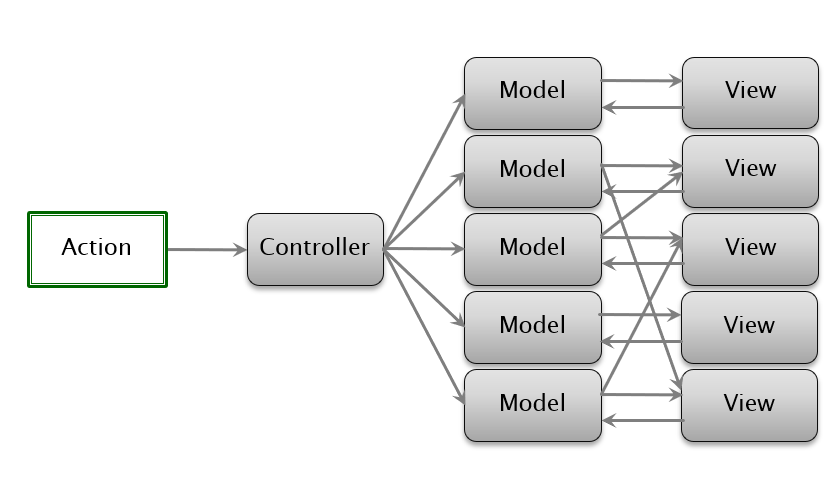
\includegraphics[width=0.6\linewidth]{assets/aula-tads-pdwa5/mvc-scalability.png}
      \end{center}
\end{frame}

\begin{frame}
      \frametitle{Framework Flux}

      \begin{itemize}
            \item O Dispatcher processa uma ação por vez.
            \item A ação é propagada para todos os armazenamentos antes das visualizações serem alteradas (evita ciclos).
            \item Se uma visualização precisa atualizar algo, ela gera uma nova ação.
      \end{itemize}
      \begin{center}
            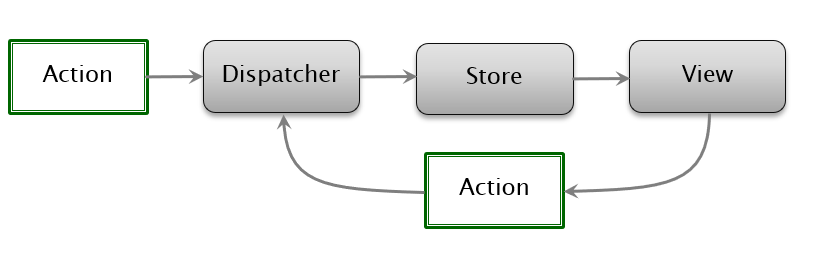
\includegraphics[width=0.8\linewidth]{assets/aula-tads-pdwa5/flux.png}
      \end{center}
\end{frame}

\begin{frame}
      \frametitle{Framework Redux}

      \begin{itemize}
            \item Sucessor informal do Flux.
            \item Todos os dados estão em um armazenamento (um objeto).
            \item Sem despachante, ações são processadas por redutor(es).
            \item O redutor é uma função pura (estado, ação) → estado.
            \item O estado nunca deve ser modificado.
      \end{itemize}
      \begin{center}
            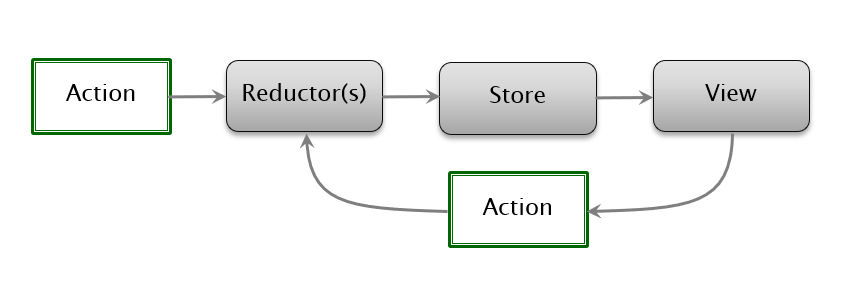
\includegraphics[width=0.8\linewidth]{assets/aula-tads-pdwa5/redux.png}
      \end{center}
\end{frame}
\begin{frame}
      \frametitle{Biblioteca UI React.js}
      
      \begin{itemize}
          \item Código aberto, impulsionado por Facebook e Instagram.
          \item Muitas vezes usado com Redux.
          \item Principais características:
          \begin{itemize}
              \item Separação de conceitos (componentes UI individuais).
              \item Fluxo de dados unidirecional.
              \item O componente filho não pode modificar seu pai.
          \end{itemize}
      \end{itemize}
      
      \end{frame}
      
      \begin{frame}
      \frametitle{Biblioteca UI React.js}
      
      \begin{itemize}
          \item Principais características (continuação):
          \begin{itemize}
              \item As ações são propagadas para cima através de callback.
              \item DOM Virtual.
              \item Alterações agregadas, então são necessárias menos modificações no DOM real quando um componente se redesenha.
              \item JSX - Extensão da linguagem Javascript.
          \end{itemize}
      \end{itemize}
      
      \end{frame}
      
      \begin{frame}
            \frametitle{React Native - Aplicações Móveis}
            
            \begin{itemize}
                \item Aplicações Móveis com Tecnologias Web:
                \begin{itemize}
                    \item Javascript e React aplicados para apps móveis.
                    \item Grande reutilização de código.
                    \item Compilado para ser um app móvel nativo.
                    \item Usa marcação especial em vez de HTML.
                    \item Pode ser combinado com código específico da plataforma.
                \end{itemize}
            \end{itemize}
            
            \end{frame}
            
            \begin{frame}
            \frametitle{React Native - Exemplo de Renderização}
            
            \begin{itemize}
                \item Exemplo de renderização:
                \begin{center}
                  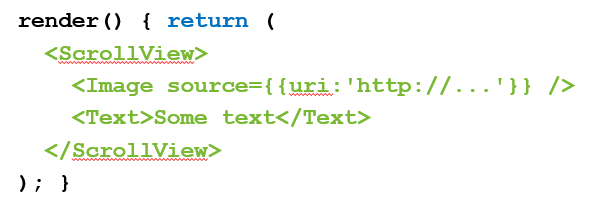
\includegraphics[width=0.8\linewidth]{assets/aula-tads-pdwa5/react-render.png}
            \end{center}
            \end{itemize}
            
            \end{frame}
            

\footlinecolor{}
\begin{frame}[fragile]{Imagem do dia}

      \begin{figure}[H]
          \centerline{
\includegraphics[width=0.8\textwidth]{assets/imagem-do-dia/single-page-application.jpg}}
          
      \end{figure}
\end{frame}
\backmatter
\end{document}
